\documentclass[12pt]{article}
\voffset=-1.5cm
\oddsidemargin=0.0cm
\textwidth = 470pt

% http://www.strath.ac.uk/aer/materials/5furtherquantitativeresearchdesignandanalysis/unit6/whatislogisticregression/

% http://www.medcalc.org/manual/logistic_regression.php


\usepackage{amsmath}
\usepackage{graphicx}
\usepackage{amssymb}
\usepackage{framed}


%----------------------------------------------------------------%

% Euclidean Distance
% Squared Euclidean Distance
% City Block Distance
%----------------------------------------------------------------%
\begin{document}
\author{Kevin O'Brien}
\Large
\title{Cluster Analysis - Distance Measures and Proximity Matrices}
\section{Hierarchial Clustering with \texttt{R}}
\tableofcontents
\newpage




\subsection{Preliminaries : The Cars Data Set}
To get an idea of what information we have in the \textbf{\textit{cars}} data set, let's look at the first few records;
{
\large
\begin{framed}
\begin{verbatim} 
> tail(cars,3)
   Country                       Car  MPG Weight Drive_Ratio
36    U.S.            Ford Mustang 4 26.5  2.585        3.08
37   Japan           Honda Accord LX 29.5  2.135        3.05
38    U.S. Ford Country Squire Wagon 15.5  4.054        2.26

   Horsepower Displacement Cylinders
36         88          140         4
37         68           98         4
38        142          351         8
> 

\end{verbatim}
\end{framed}
}
\newpage
{
\large
\begin{verbatim}
> summary(cars)
    Country                      Car          MPG            Weight     
        : 0   AMC Concord D/L      : 1   Min.   :15.50   Min.   :1.915  
 France : 1   AMC Spirit           : 1   1st Qu.:18.52   1st Qu.:2.208  
 Germany: 5   Audi 5000            : 1   Median :24.25   Median :2.685  
 Italy  : 1   BMW 320i             : 1   Mean   :24.76   Mean   :2.863  
 Japan  : 7   Buick Century Special: 1   3rd Qu.:30.38   3rd Qu.:3.410  
 Sweden : 2   Buick Estate Wagon   : 1   Max.   :37.30   Max.   :4.360  
 U.S.   :22   (Other)              :32                        
           
  Drive_Ratio      Horsepower     Displacement     Cylinders    
 Min.   :2.260   Min.   : 65.0   Min.   : 85.0   Min.   :4.000  
 1st Qu.:2.695   1st Qu.: 78.5   1st Qu.:105.0   1st Qu.:4.000  
 Median :3.080   Median :100.0   Median :148.5   Median :4.500  
 Mean   :3.093   Mean   :101.7   Mean   :177.3   Mean   :5.395  
 3rd Qu.:3.625   3rd Qu.:123.8   3rd Qu.:229.5   3rd Qu.:6.000  
 Max.   :3.900   Max.   :155.0   Max.   :360.0   Max.   :8.000  
\end{verbatim}
}
\newpage

%http://www.econ.upf.edu/~michael/stanford/maeb4.pdf
%http://stn.spotfire.com/spotfire_client_help/hc/hc_distance_measures_overview.htm
\subsection{Distance Matrices}
In clustering analysis, an important step is calculating a \textbf{distance matrix}. \\ For a data set with n observations, the distance matrix will have $n$ rows and $n$ columns; the $(i,j)$th element of the distance matrix will be the ``distance" between observation i and observation j.
\begin{itemize}
	\item There are two functions that can be used to calculate distance matrices in \texttt{R}; 
	\begin{itemize}
		\item the \texttt{dist} function, 
		\item  the \texttt{daisy} function, which is part of the \textbf{\textit{cluster}} library. 
	\end{itemize}
	\item We'll use the \texttt{dist} function from now on in this example.
	%\item Additionally you should familiarize yourself with the \texttt{daisy} function, since it offers some capabilities that \texttt{dist} does not. 
	\item Each function provides a choice of distance metrics; in this example, we'll use the default of \textbf{\textit{Euclidean}} distance, but you may find that using other metrics will give different insights into the structure of your data.
\end{itemize} 
\newpage
\begin{framed}
	\begin{verbatim}
	cars.dist = dist(cars)
	\end{verbatim}
\end{framed}

\begin{verbatim}
1          2          3          4          5          6         ....         
2  7.67122038                                                                                        
3  7.83892209 1.22909204                                                                             
4  7.93329268 1.17056831 0.32148633                                                                  
5  7.79786438 1.24693030 0.09318086 0.35340761                                                       
6  7.84972498 1.19468213 0.24363662 0.27248979 0.21846778                                            
7  7.78735704 0.52646180 1.16777805 0.98623148 1.17782394 1.06988927
...........
\end{verbatim}

\newpage
\subsubsection*{Remarks on the Distance Matrix}
\begin{itemize}
	\item If you display the distance matrix in \texttt{R} (for example, by typing its name), you'll notice that only the lower triangle of the matrix is displayed. 
	\item This is to remind us that the distance matrix is symmetric, since it doesn't matter which observation we consider first when we calculate a distance. \texttt{R} takes advantage of this fact by only storing the lower triangle of the distance matrix. 
	\item All of the clustering functions will recognize this and have no problems, but if you try to access the distance matrix in the usual way (for example, with subscripting), you'll see an error message. 
	\item If you need to use the distance matrix with anything other than the clustering functions, you'll need to use \texttt{as.matrix() }to convert it to a regular matrix.
\end{itemize}
\newpage
\subsection{Euclidean Distance}
The Euclidean Distance between two points, x and y, with $k$ dimensions is calculated as:
\[ \sqrt{ \sum^{k}_{j=1} ( x_j - y_j)^2 } \]
The Euclidean distance is always greater than or equal to zero. The measurement would be zero for identical points and high for points that show little similarity.

\subsubsection{Example}
Compute the Euclidean Distance between the following points:
$X = \{1,5,4,3\}$ and $Y = \{2,1,8,7\}$

\begin{center}
	\begin{tabular}{|c|c|c|c|}
		\hline
		$x_j$	&	$y_j$	&   $x_j - y_j$	&	$(x_j - y_j)^2$	\\ \hline
		1	&	2	&	-1	&	1	\\
		5	&	1	&	4	&	16	\\
		4	&	8	&	-4	&	16	\\
		3	&	7	&	-4	&	16	\\ \hline
		&		&		&	49	\\ \hline
	\end{tabular}
\end{center}
The Euclidean Distance between the two points is $\sqrt{49}$ i.e. 7.

\subsection{Squared Euclidean Distance}
The Squared Euclidean distance between two points, x and y, with $k$ dimensions is calculated as:
\[ \sum^{k}_{j=1} ( x_j - y_j)^2  \]
The Squared Euclidean distance may be preferred to the Euclidean distance as it is slightly less computational complex, without loss of any information.

%---------------------------------------------------------------------------%
\newpage
\subsubsection{{\large Standardized Euclidean distance}}

Let us consider measuring the distances between between two points using
the three continuous variables pollution, depth and temperature. Let us suppose that a difference of 4.1 in terms of pollution is considered quite large and unusual, while a difference of 48 in terms of depth is large, but not particularly unusual.
What would happen if we applied the Euclidean distance formula to measure distance between two cases.
\begin{center}
	\begin{tabular}{|c|c|c|}
		\hline
		% after \\: \hline or \cline{col1-col2} \cline{col3-col4} ...
		Variables & case 1 & case 2 \\ \hline 
		Pollution & 6.0 & 1.9 \\
		Depth & 51 & 99 \\
		Temp & 3.0 & 2.9 \\
		\hline
	\end{tabular}
\end{center}

\noindent Here is the calculation for Euclidean Distance:
\[ d = \sqrt{(6.0 - 1.9)^2 + (51 - 99)^2 + (3.0 - 2.9)^2}   \]
\[ d = \sqrt{16.81 + 2304 + 0.01} = \sqrt{2320.82} = 48.17 \]
\noindent The contribution of the second variable depth to this calculation is huge. You could say
that the distance is practically just the absolute difference in the depth values (equal to
$|51-99| = 48$) with only tiny additional contributions from pollution and temperature. 


These three variables are on
completely different scales of measurement and the larger depth values have larger differences, so they will dominate in the calculation of Euclidean distances.
\newpage

%========================================================================== %
\begin{itemize}
\item The approach to take here is \textbf{standardization}, which is is necessary to balance out the contributions, and the
conventional way to do this is to transform the variables so they all have the same variance
of 1. 
\item At the same time we \textbf{\textit{center}} the variables at their means
\item This centering is not
necessary for calculating distance, but it makes the variables all have mean zero and thus
easier to compare. 

\item  The transformation commonly called standardization is thus as follows:
\end{itemize}


\[\mbox{standardized value} = \frac{\mbox{observed value - mean}}{ \mbox{standard deviation}}\]
\begin{center}
	\begin{tabular}{|c|c|c|c|c|c|c|}
		\hline
		% after \\: \hline or \cline{col1-col2} \cline{col3-col4} ...
		Variables & Case 1 & Case 2 & Mean & Std. Dev & Case 1 (std) & Case 2 (std) \\ \hline
		Pollution & 6.0 & 1.9 & 4.517	&	2.141	&	0.693	&	-1.222	\\
		Depth & 51 & 99 & 74.433	&	15.615	&	-1.501	&	1.573	\\
		Temp & 3.0 & 2.9 & 3.057	&	0.281	&	-0.201	&	-0.557	\\
		\hline
	\end{tabular}
\end{center}

\[ d_{std} =  \sqrt{(0.693 - (- 1.222))^2 + (-1.501-1.573)^2 + (-0.201-(-0.557))^2} \]

\[ d_{std} = \sqrt{3.667 + 9.449 + 0.127} = \sqrt{13.243} = 3.639 \]
\newpage
\begin{itemize}
\item Pollution and temperature have higher contributions than before but depth still plays the
largest role in this particular example, even after standardization. 
\item But this contribution is
justified now, since it does show the biggest standardized difference between the samples. 

\end{itemize}
%--------------------------------------------------------------------------------------%
\newpage
\subsection{Manhattan (City Block) Distance}
The City block distance between two points, x and y, with $k$ dimensions is calculated as:
\[ \sum^{k}_{j=1} | x_j - y_j |  \]

\noindent The City block distance is always greater than or equal to zero. The measurement would be zero for identical points and high for points that show little similarity.

\subsubsection{{\large Example}}
Compute the Manhattan Distance between the following points: 
$X = \{1,3,4,2\}$ and $Y = \{5,2,5,2\}$


\begin{center}
	\begin{tabular}{|c|c|c|c|}
		\hline
		$x_j$	&	$y_j$	&   $x_j - y_j$	&	$| x_j - y_j |$	\\ \hline
		1	&	5	&	-4	&	4	\\
		3	&	2	&	1	&	1	\\
		4	&	5	&	-1	&	1	\\
		2	&	2	&	0	&	0	\\ \hline
		& & & 6 \\
		\hline
	\end{tabular}
\end{center}
The Manhattan Distance between the two points is 6.
\newpage
\subsection{Standardization - The \texttt{scale} Function}
\begin{itemize}
\item It is clear that the variables are measured on different scales, so we will likely want to standardize the data before proceeding. 
\item The \texttt{daisy} function in the \textbf{\textit{cluster}} library will automatically perform standardization, but it doesn't allow the user complete control. 
\bigskip

\item If you have a particular method of standardization in mind, you can use the \texttt{scale} function. You pass to the scale function a matrix or data frame to be standardized, and two optional vectors. 
\item The first, called \texttt{center}, is a vector of values, one for each column of the matrix or data frame to be standardized, which will be subtracted from every entry in that column. 
\item The second, called \texttt{scale}, is similar to \texttt{center}, but is used to divide the values in each column. In order to get z-scores, you could pass scale a vector of means for center, and a vector of standard deviations for scale.

\item \textbf{Defaults}: The default settings for \texttt{center} and \texttt{scale} are the mean and standard deviation respectively. \\ However, implicit in this choice is the \textbf{\textit{assumption of normally distributed data}}.
 
\item These vectors can be created with the \texttt{apply} function, that performs the same operation on each row or column of a matrix.\\ 
\item 
\textit{(Remark, for a column-wise operation with the \texttt{apply} function, specify the addition argument ``2", Otherwise it would work on a row-wise basis)}
\item Non-numeric variables, such as the country of origin and name of the car, will not be useful in the cluster analysis, so they have been removed. \\ The number of cylinders has been retained as a variable.
\end{itemize}

\newpage
\noindent \textbf{The \texttt{scale()} function - Example:} \\ Suppose we want to standardize by subtracting the median (\texttt{median}) and dividing by the mean average deviation (\texttt{mad}):
\begin{framed}
\begin{verbatim}
# First, remove the first two (non-numeric) columns.
cars.use = cars[,-c(1,2)]  

# Compute the medians of each column
medians = apply(cars.use,2,median)

# Compute the MADs of each column
mads = apply(cars.use,2,mad)

# Use the scale function
cars.use = scale(cars.use,center=medians,scale=mads)
\end{verbatim}
\end{framed}
\newpage
\begin{verbatim}
> head(cars.use)
         MPG     Weight Drive_Ratio Horsepower Displacement
1 -0.8402554  2.0921704  -0.4918162  1.5785954    2.6912849
2  1.2403771 -0.9617739  -0.1545708 -0.5740347   -0.6744908
3  0.8745516 -0.9492833   0.9836324 -0.8323503   -0.7946970
4  1.1260566 -0.8868304   0.9133729 -1.0045607   -0.8347658
5  0.8288234 -0.8680946   0.9836324 -0.8323503   -0.7946970
6  0.8631195 -0.8306229   0.8712172 -1.0045607   -0.8481220
   Cylinders
1  4.7214353
2 -0.6744908
3 -0.6744908
4 -0.6744908
5 -0.6744908
6 -0.6744908

\end{verbatim}
\begin{itemize} 
%\item The \texttt{scale} function doesn't change the order of the rows of the data frame, so it will be easy to identify observations using the omitted columns from the original data.
\item We will continue the workshop, using both scaled and unscaled data, for the sake of simplicity.
\end{itemize} 

%--------------------------------------------------------------------------------------%
\newpage
\subsection{{\large Cluster Analysis : Proximity Matrices}}

Using \textbf{\textit{nearest neighbour}} linkage, describe how the agglomeration schedule based on the following 
proximity matrix. With nearest neighbour, a case is assigned to the cluster of the case with which it has the shortest distance. Cluster are also joined on this basis.


% latex table generated in R 2.15.2 by xtable 1.7-1 package
% Tue May 14 19:17:33 2013
{

\begin{table}[ht]
	\centering
		\large
	\begin{tabular}{|r|rrrrrrrrrr|}
		\hline
		Case & 1 & 2 & 3 & 4 & 5 & 6 & 7 & 8 & 9 & 10 \\
		\hline
		1 & 0.00 & \textbf{4.82} & 89.39 & 85.97 & 46.26 & 71.87 & 56.42 & 23.75 & 31.57 & 11.70 \\
		2 & \textbf{4.82} & 0.00 & 94.24 & 38.96 & \textbf{5.55} & 35.07 & 74.52 & 71.27 & 61.84 & \textbf{4.84} \\
		3 & 89.39 & 94.24 & 0.00 & 57.65 & 27.27 & 25.31 & 20.89 & \textbf{2.84} & 63.50 & 89.39 \\
		4 & 85.97 & 38.96 & 57.65 & 0.00 & \textbf{22.94} & \textbf{7.13} & 70.49 & 23.09 & \textbf{12.75} & 85.97 \\
		5 & 46.26 & \textbf{5.55} & 27.27 & \textbf{22.94} & 0.00 & 39.44 & 17.43 & 79.22 & 14.47 & 46.26 \\
		6 & 71.87 & 35.07 & 25.31 & \textbf{7.13} & 39.44 & 0.00 & 27.50 & 30.65 & 13.34 & 71.87 \\
		7 & 56.42 & 74.52 & 20.89 & 70.49 & 17.43 & 27.50 & 0.00 & 91.16 & 44.92 & \textbf{6.42} \\
		8 & 23.75 & 71.27 & \textbf{2.84} & 23.09 & 79.22 & 30.65 & 91.16 & 0.00 & \textbf{3.18} & 23.75 \\
		9 & 31.57 & 61.84 & 63.50 & \textbf{12.75} & 14.47 & 13.34 & 44.92 & \textbf{3.18} & 0.00 & 31.57 \\
		10 & 11.70 & \textbf{4.84} & 89.39 & 85.97 & 46.26 & 71.87 & \textbf{6.42} & 23.75 & 31.57 & 0.00 \\
		\hline
	\end{tabular}
\end{table}
}

\begin{itemize}
	\item The closest pair in terms of distance (2.84) are cases 3 and 8. So this is the first linkage.
	\item The next closest pair (3.18) are 8 and 9. The next linkage joins case 9 to 3 and 8.
	\item The next closest pair (4.82) are 1 and 2. So this is the next linkage. [ So far (3,8,9) and (2,10) ] 
	\item The next closest pair (4.84) are 2 and 10. The next linkage joins case 1 to 2 and 10.
	\item The next closest pair (5.55) are 2 and 5. The next linkage joins case 5 to 1, 2 and 10. [ So far (3,8,9) and (1,2,5,10)]
	\item The next closest pair (6.42) are 7 and 10. The next linkage joins case 7 to 1, 2, 5 and 10.
	\item The next closest pair (7.13) are 4 and 6. The next linkage joins case 4 to 6. [ So far (3,8,9), (4,6) and (1,2,5,10) All cases are in clusters. This is a 3 cluster solution. ]
	\item The next closest pair (11.70) are 1 and 10. Disregard, because they are already clustered together.
	\item The next closest pair (19.44) are 4 and 9. This joins cluster (4,6) to cluster (3,8,9) [ So far (3,4,6,8,9) and (1,2,5,10). This is a 2 cluster solution.]
	\item The next closest pairing is 4 and 5. This linkage joins all cases together in one cluster.
\end{itemize}
\newpage

\subsection{Implementation of the Clustering Analysis}
To get started, we'll use the \texttt{hclust} method. The argument to this function is the distance matrix that we have created earlier.
%(The \textbf{\textit{cluster}} library provides a similar function, called \texttt{agnes}, to perform hierarchical cluster analysis.)
\begin{framed}
	\begin{verbatim}
	cars.hclust = hclust(cars.dist)
	
	cars.hclust
	
	names(cars.hclust)
	\end{verbatim}
\end{framed}


\begin{itemize} 
	\item We are going to use the default method of \texttt{hclust}, which is to update the distance matrix using what \texttt{R} calls \textbf{\textit{complete linkage}}. 
	\item Using this method, when a cluster is formed, its distance to other objects is computed as the maximum distance between any object in the cluster and the other object. 
	\item Other linkage methods will provide different solutions, and \textbf{should not} be ignored. 
	\item For example, using \textbf{\textit{Ward's Linkage}} (\texttt{method=ward}) tends to produce clusters of fairly equal size, and can be useful when other methods find clusters that contain just a few observations.
\end{itemize}
 
%\textit{\subsection{Hierarchical Clustering Analysis} 
%First, we'll take a look at a hierarchical method, since it will provide information about solutions with different numbers of clusters. }
%------------------------------------------------------ %

\newpage
\subsection{Agglomeration Methods used by \texttt{hclust}}
\begin{itemize}
\item The agglomeration method used by \texttt{hclust} can be specified using the \texttt{method=} argument.
\item The default method is \texttt{complete linkage}.

\item The other agglomeration methods are
\begin{framed}
\begin{description}
\item[\texttt{single }]: nearest neighbor
\item[\texttt{complete }]: furthest neighbor or compact (\textit{default})
\item[\texttt{ward.D }]:  Ward's minimum variance method
\item[\texttt{ward.D2}]:  Ward's minimum variance method \\ (\textit{alternative computation})
\item[\texttt{mcquitty }]: McQuitty's method
\item[\texttt{average }]: average similarity
\item[\texttt{median }]: median (as opposed to average) similarity
\item[\texttt{centroid }]: geometric centroid
\item[\texttt{flexible }]: flexible Beta
\end{description}
\end{framed}
\end{itemize}
\newpage
\subsection{Dendrograms}
\begin{itemize}
\item The main graphical tool for looking at a hierarchical cluster solution is known as a dendrogram. 
\item A dendrogram is a tree-structured graph used in heat maps to visualize the result of a hierarchical clustering calculation. 
\item The dendrogram lists the objects which are clustered along the x-axis, and the distance at which the cluster was formed along the y-axis. \\ \textit{(Distances along the x-axis are not particularly meaningful in a dendrogram; the observations are often equally spaced to make the dendogram easier to read.) 
}
\item 
The result of a clustering is presented either as the distance or the similarity between the clustered rows or columns depending on the selected distance measure. 
\item  
When you use \texttt{hclust} (or \texttt{agnes}) to perform a cluster analysis, you can see the dendrogram by passing the result of the clustering to the \texttt{plot} function.
\item 
To illustrate interpretation of the dendrogram, we'll look at a cluster analysis performed on the cars data set.
\end{itemize}
%To create a dendogram from a cluster solution, simply pass it to the plot function. The result is displayed below.
\newpage
\begin{framed}
\begin{verbatim}
plot(cars.hclust)
plot(cars.hclust,labels=cars$Car)
\end{verbatim}
\end{framed}
\newpage
\begin{figure}[h!]
\centering
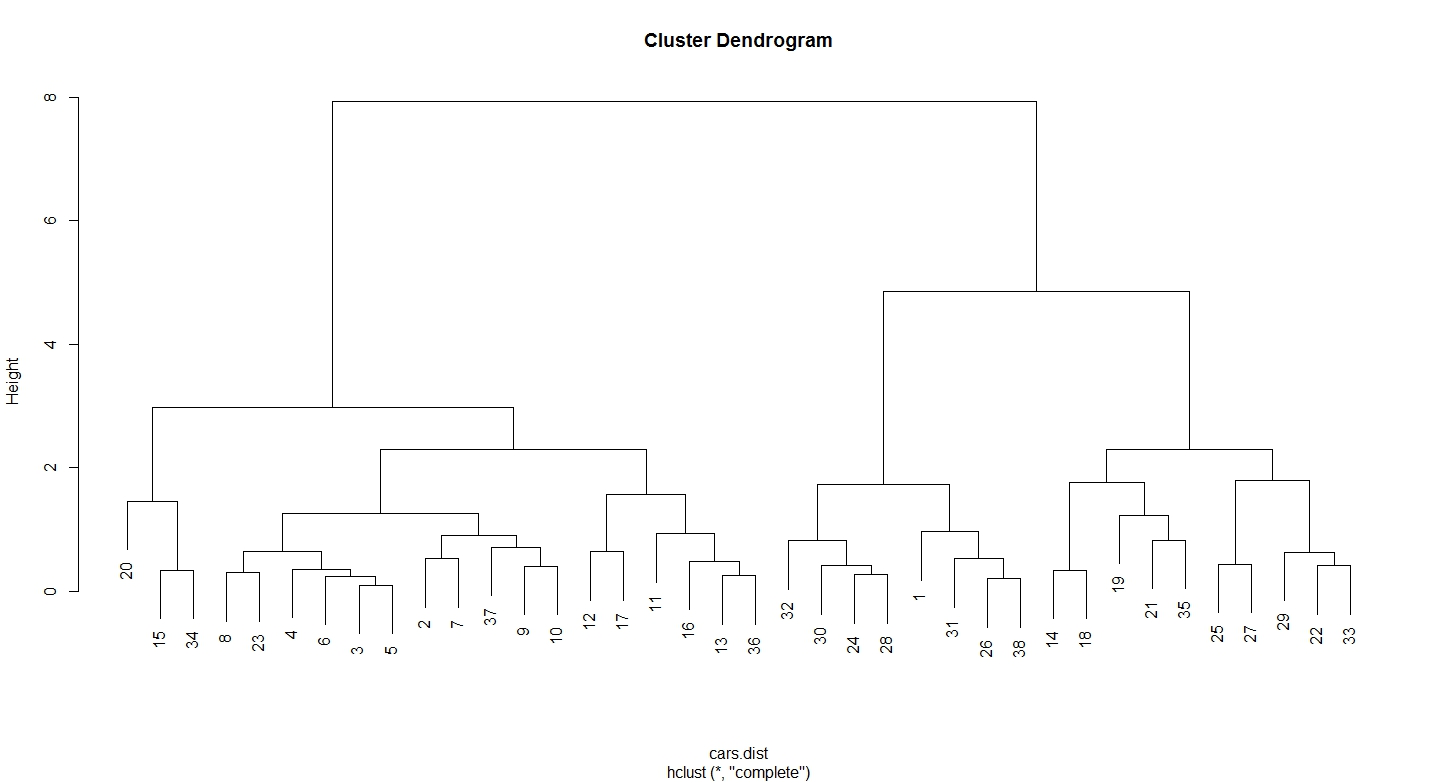
\includegraphics[width=0.9\linewidth]{./Carsdendro1}

\label{fig:Carsdendro1}
\end{figure}
\begin{figure}[h!]
\centering
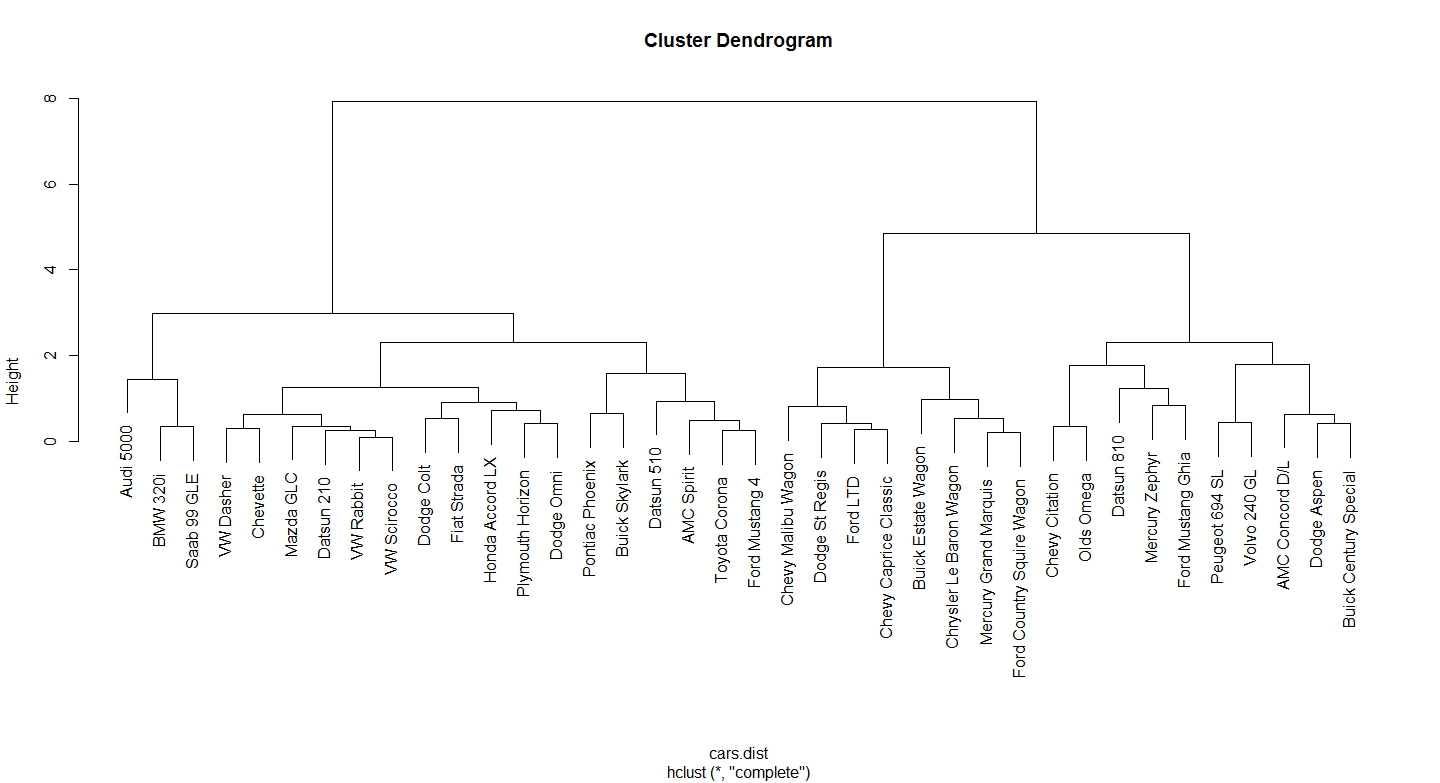
\includegraphics[width=0.9\linewidth]{./Carsdendro2}

\label{fig:Carsdendro2}
\end{figure}

\begin{itemize}
\item If you choose any height along the y-axis of the dendrogram, and move across the dendrogram counting the number of lines that you cross, each line represents a group that was identified when objects were joined together into clusters.
\item  The observations in that group are represented by the branches of the dendrogram that spread out below the line.
\item  For example, if we look at a height of 6, and move across the x-axis at that height, we'll cross two lines. That defines a two-cluster solution; by following the line down through all its branches, we can see the names of the cars that are included in these two clusters. 
\item Since the y-axis represents how close together observations were when they were merged into clusters, clusters whose branches are very close together (in terms of the heights at which they were merged) probably aren't very reliable. But if there's a big difference along the y-axis between the last merged cluster and the currently merged one, that indicates that the clusters formed are probably doing a good job in showing us the structure of the data.
\end{itemize}

\newpage
\begin{itemize}
\item  Looking at the dendrogram for the car data, there are clearly two very distinct groups; the right hand group seems to consist of two more distinct cluster, while most of the observations in the left hand group are clustering together at about the same height.
\item For this data set, it looks like either two or three groups might be an interesting place to start investigating. 
\item This is not to imply that looking at solutions with more clusters would be meaningless, but the data seems to suggest that two or three clusters might be a good start.
\item For a problem of this size, we can see the names of the cars, so we could start interpreting the results immediately from the dendrogram, but when there are larger numbers of observations, this won't be practical.
\end{itemize}
\newpage
\subsection{Using the \texttt{rect.hclust} Command}

\begin{itemize}
	\item  This command is used to draw rectangles around the branches of a dendrogram highlighting the corresponding clusters. First the dendrogram is cut at a certain level, then a rectangle is drawn around selected branches.
	\item \textbf{Simple Demontration,}
	\begin{itemize}
		\item using cars (unscaled)
		\item Linkage Method : Ward's Linkage
	\end{itemize}
\end{itemize}

{
	\Large
	\begin{framed}
		\begin{verbatim}
		plot(hclust(cars.dist,method="ward.D"))
		rect.hclust(hclust(cars.dist,method="ward.D"),h=300)                                            
		\end{verbatim}
	\end{framed}
}
\newpage
\begin{figure}[h!]
	\centering
	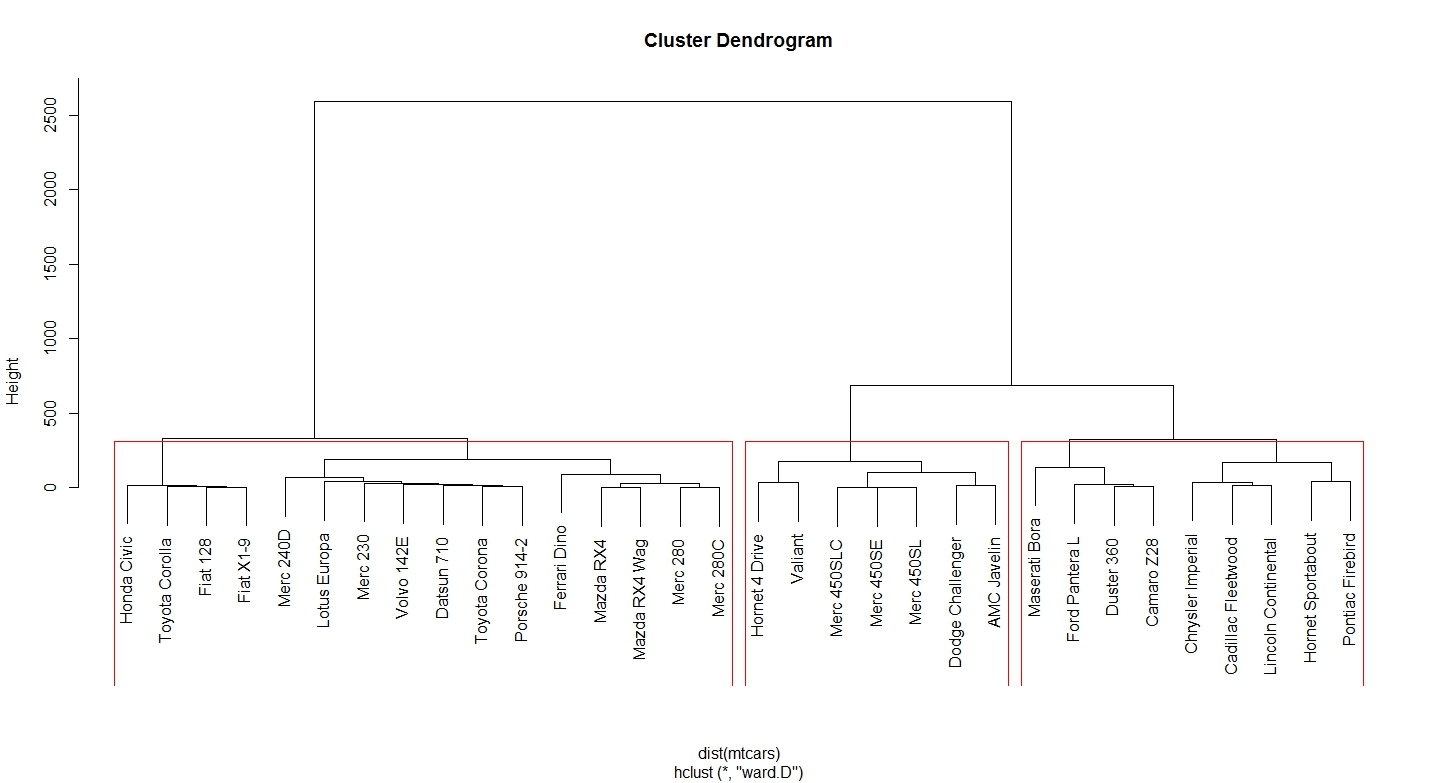
\includegraphics[width=1.09\linewidth]{./rectclust1}
\end{figure}







\newpage
\subsection{Using the \texttt{cutree} Command}
\begin{itemize}
\item One of the first things we can look at is how many cars are in each of the groups. Suppose that we would like to do this for both the two cluster and three cluster solutions. 
\item You can create a vector showing the cluster membership of each observation by using the \texttt{cutree} function. 
\item Since the object returned by a hierarchical cluster analysis contains information about solutions with different numbers of clusters, we pass the \texttt{cutree} function the cluster object and the number of clusters we're interested in.

\item  So to get cluster memberships for the three cluster solution, we could use:
\end{itemize}
\newpage
\begin{framed}
\begin{verbatim}
groups.3 = cutree(cars.hclust,3)
\end{verbatim}
\end{framed}

\begin{verbatim}
> groups.3 = cutree(cars.hclust,3)
>
> groups.3
 1  2  3  4  5  6  7  8  9 10 11 12 13 14 15 
 1  2  2  2  2  2  2  2  2  2  2  2  2  3  2 
16 17 18 19 20 21 22 23 24 25 26 27 28 29 30 
 2  2  3  3  2  3  3  2  1  3  1  3  1  3  1 
31 32 33 34 35 36 37 38 
 1  1  3  2  3  2  2  1 
>
> table(groups.3)
groups.3
 1  2  3 
 8 20 10 
>
> groups.4 = cutree(cars.hclust,4)
>
> table(groups.4)
groups.4
 1  2  3  4 
 8 17 10  3 
\end{verbatim}


\newpage
\subsubsection*{Automating the Process using \texttt{sapply}}
\begin{itemize}
\item We'd like a solution where there aren't too many clusters with just a few observations, because it may make it difficult to interpret our results. 
\item For the three cluster solution, the distribution among the clusters looks satisfactory.


\item You can get this information for many different groupings at once by combining the calls to \texttt{cutree()} and table in a call to \texttt{sapply()}. 
\item For example, to see the sizes of the clusters for solutions ranging from 2 to 6 clusters, we could use:
\end{itemize} 
\newpage
\begin{framed}
\begin{verbatim}
ClusSize=function(ncl=2) {
 table(cutree(cars.hclust,ncl))
 }
counts = sapply(2:6,ClusSize)
names(counts) = 2:6
counts
\end{verbatim}
\end{framed}
\begin{verbatim}
$"2"

 1  2
18 20

$"3"

 1  2  3
 8 20 10


......

\end{verbatim}
\newpage
\subsection*{Cluster Membership}
\begin{itemize}
\item To see which cars are in which clusters, we can use subscripting on the vector of car names to choose just the observations from a particular cluster. 
\item Since we used all of the observations in the data set to form the distance matrix, the ordering of the names in the original data will coincide with the values returned by cutree. 
\item If observations were removed from the data before the distance matrix is computed, it's important to remember to make the same deletions in the vector from the original data set that will be used to identify observations. 
\item So, to see which cars were in the first cluster for the four cluster solution, we can use:
{
\large
\begin{framed}
\begin{verbatim}
> cars$Car[groups.3 == 1]
[1] Buick Estate Wagon        Ford Country Squire Wagon
[3] Chevy Malibu Wagon        Chrysler LeBaron Wagon
[5] Chevy Caprice Classic     Ford LTD
[7] Mercury Grand Marquis     Dodge St Regis
\end{verbatim}
\end{framed}
}
\end{itemize}

\newpage
\subsection*{Cross-Tabulations}
\begin{itemize}
\item Cluster analysis is often performed to see if observations naturally group themselves in accord with some already measured variable. 
\item For the \textbf{\textit{cars}} data set, we could ask whether the clusters reflect the country of origin of the cars, stored in the variable \texttt{Country} in the original data set. 
\item The \texttt{table} function can be used, this time passing two arguments, to produce a cross-tabulation of cluster group membership and country of origin:
\end{itemize}
\begin{framed}
\begin{verbatim}
> table(groups.3,cars$Country)

groups.3 France Germany Italy Japan Sweden U.S.
       1      0       0     0     0      0    8
       2      0       5     1     6      1    7
       3      1       0     0     1      1    7
>                                                 
\end{verbatim}
\end{framed}
\end{document}
Of interest is the fact that all of the cars in cluster 1 were manufactured in the US. Considering the state of the automobile industry in 1978, and the cars that were identified in cluster 1, this is not surprising.
In an example like this, with a small number of observations, we can often interpret the cluster solution directly by looking at the labels of the observations that are in each cluster. Of course, for larger data sets, this will be impossible or meaningless. A very useful method for characterizing clusters is to look at some sort of summary statistic, like the median, of the variables that were used to perform the cluster analysis, broken down by the groups that the cluster analysis identified. The aggregate function is well suited for this task, since it will perform summaries on many variables simultaneously. Let's look at the median values for the variables we've used in the cluster analysis, broken up by the cluster groups. One oddity of the aggregate function is that it demands that the variable(s) used to divide up the data are passed to it in a list, even if there's only one variable:
\begin{framed}
\begin{verbatim}
> aggregate(cars.use,list(groups.3),median)
  Group.1        MPG     Weight Drive_Ratio Horsepower Displacement  Cylinders
1       1 -0.7945273  1.5051136  -0.9133729  1.0476133    2.4775849  4.7214353
2       2  0.6859228 -0.5870568   0.5269459 -0.6027364   -0.5809970 -0.6744908
3       3 -0.4058377  0.5246039  -0.1686227  0.3587717    0.3272282  2.0234723

\end{verbatim}
\end{framed}
If the ranges of these numbers seem strange, it's because we standardized the data before performing the cluster analysis. While it is usually more meaningful to look at the variables in their original scales, when data is centered, negative values mean "lower than most" and positive values mean "higher than most". Thus, group 1 is cars with relatively low MPG, high weight, low drive ratios, high horsepower and displacement, and more than average number of cylinders. Group 2 are cars with high gas mileage, and low weight and horsepower; and group 3 is similar to group 1. It may be easier to understand the groupings if we look at the variables in their original scales:
\begin{framed}
\begin{verbatim}
> aggregate(cars[,-c(1,2)],list(groups.3),median)
  Group.1   MPG Weight Drive_Ratio Horsepower Displacement Cylinders
1       1 17.30  3.890       2.430      136.5          334         8
2       2 30.25  2.215       3.455       79.0          105         4
3       3 20.70  3.105       2.960      112.5          173         6
\end{verbatim}
\end{framed}

It may also be useful to add the numbers of observations in each group to the above display. Since aggregate returns a data frame, we can manipulate it in any way we want:
\begin{framed}
\begin{verbatim}
> a3 = aggregate(cars[,-c(1,2)],list(groups.3),median)
> data.frame(Cluster=a3[,1],Freq=as.vector(table(groups.3)),a3[,-1])
  Cluster Freq   MPG Weight Drive_Ratio Horsepower Displacement Cylinders
1       1    8 17.30  3.890       2.430      136.5          334         8
2       2   20 30.25  2.215       3.455       79.0          105         4
3       3   10 20.70  3.105       2.960      112.5          173         6
\end{verbatim}
\end{framed}
To see how the four cluster solution differed from the three cluster solution, we can perform the same analysis for that solution:
\begin{framed}
\begin{verbatim}
> a4 = aggregate(cars[,-c(1,2)],list(groups.4),median)
> data.frame(Cluster=a4[,1],Freq=as.vector(table(groups.4)),a4[,-1])
  Cluster Freq  MPG Weight Drive_Ratio Horsepower Displacement Cylinders
1       1    8 17.3  3.890        2.43      136.5          334         8
2       2   17 30.9  2.190        3.37       75.0           98         4
3       3    3 21.5  2.795        3.77      110.0          121         4
4       4   10 20.7  3.105        2.96      112.5          173         6
\end{verbatim}
\end{framed}

The main difference seems to be that the four cluster solution recognized a group of cars that have higher horsepower and drive ratios than the other cars in the cluster they came from.
\newpage

\end{document}